\documentclass[twoside]{homework}

\usepackage{dsfont} 
\usepackage{graphicx}

\studname{Si Kai Lee}
\uni{sl3950}
\studmail{sl3950@columbia.edu}
\coursename{Foundations of Graphical Models}
\hwNo{1}

\begin{document}
\maketitle

\section*{Problem 1}
\subsection*{a}
$2^6 = 64$
\subsection*{b}
According to the readings, size of table of conditional probability associated with node $X_i = r^{m_i + 1}$ where $m_i$ are the number of variables conditioned on. $P(X_1 | X_2, X_3, X_4) = 2^{3+1} = 16$.
\subsection*{c}
$P(X_1, X_2 | X_3, X_4, X_5) = 2^{4+1} = 32$
\subsection*{d}
$p(x_{1:6}) = p(x_6).p(x_5 | x_6) p(x_4 | x_6) p(x_3) p(x_2 | x_3, x_4, x_5) p(x_1 | x_2, x_3)$
\subsection*{e}
The number of entries are (w.r.t. to the above factorisation) is $2 + 2^2 + 2^2 + 2 + 2^4 + 2^3 = 36$
\subsection*{f}
$P(X_1 | X_2, X_3, X_4)  = P(X_1 | X_2, X_3)$ as $X_1 \!\perp\!\!\!\perp X_4 | \{X_2, X_3\}$ . Hence we will touch $2^3 = 8$ entries.
\subsection*{g}
$P(X_1, X_2 | X_3, X_4, X_5)  = \sum_{X_3} P(X_1 | X_2, X_3) P(X_2 | X_3, X_4, X_5)$. Hence we will touch $2^3 +2 ^4 = 24$ entries.

\section*{Problem 2}
\subsection*{a}
We redraw the affected nodes in the following manner:\\
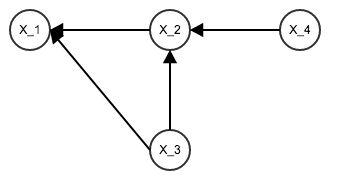
\includegraphics[scale=0.5]{2a}\\
Then we can see that $X_1\not\!\perp\!\!\!\perp X_4$
\subsection*{b}
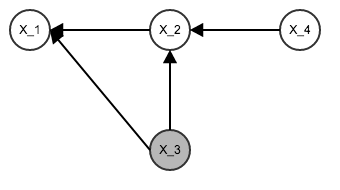
\includegraphics[scale=0.5]{2b}\\
From the diagram, it is obvious that that $X_1\not\!\perp\!\!\!\perp X_4 | X_3$
\subsection*{c}
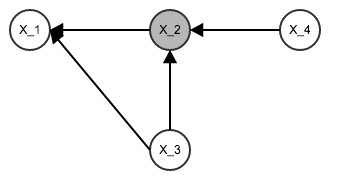
\includegraphics[scale=0.5]{2c}\\
We can have a ball going from $X_1$ to $X_3$ to $X_2$ and then $X_1$, hence $X_1\not\!\perp\!\!\!\perp X_4 | X_2$
\subsection*{d}
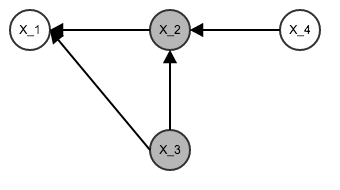
\includegraphics[scale=0.5]{2d}\\
Balls are not permitted to go from $X_1$ to either $X_2$ and $X_3$ or from $X_4$ to $X_3$ to $X_1$ so $X_1\!\perp\!\!\!\perp X_4 | X_2, X_3$
\subsection*{e}
Although we have a v-structure between $X_3, X_2, X_4$, we have an inverted v-structure between $X_3, X_1, X_2$. We then go from $X_3$ to $X_2$ via $X_1$ then to $X_4$ which gives $X_3 \not\!\perp\!\!\!\perp X_4$
\subsection*{f}
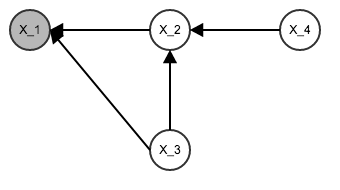
\includegraphics[scale=0.5]{2f}\\
We cannot have a ball going from $X_3$ to $X_2$ via $X_1$ as $X_1$ is now shaded thus $X_3 \!\perp\!\!\!\perp X_4 | X_1$
\subsection*{g}
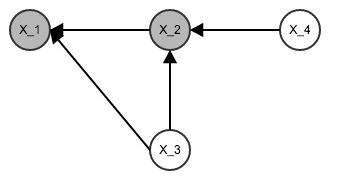
\includegraphics[scale=0.5]{2g}\\
We can have a ball going from $X_3$ to $X_4$ via $X_2$ thus $X_3 \not\!\perp\!\!\!\perp X_4 | X_1, X_2$

\section*{Problem 3}
\subsection*{a}
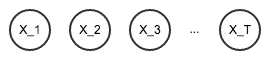
\includegraphics[scale=0.5]{3a}
\subsection*{b}
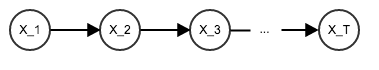
\includegraphics[scale=0.5]{3b}
\subsection*{c}
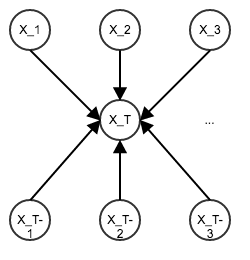
\includegraphics[scale=0.5]{3c}
\subsection*{d}
All nodes in a) are independent on each other, the $i^{th}$ node in b) is only dependent on the $i-1^{th}$ node and the $T^{th}$ node is dependent on all nodes in c).

We could model coin flips with a), speech with b) and the indicator function that all items on this week's shopping list have been bought $(X_T$) with c) and $X_1 ... X_T$ being all ingredients needed. 

\section*{Problem 4}
\subsection*{a}
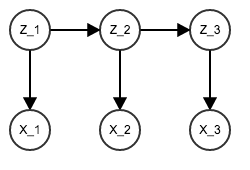
\includegraphics[scale=0.5]{4a}
\subsection*{b}
We begin by converting the HMM to a tree by hanging the graph on the node representing the hidden state we want to marginalise and pass messages from the leaves to the root to obtain the marginal probability of the node. A good ordering can be obtained by performing a depth-first search on the node we want to marginalise which would ensure that we do not do any unnecessary calculations. Since we are marginalising on $z_2$, have $I = \{x_1, z_1, x_2, x_3, z_3, z_2\}$. 
\subsection*{c}
The outcome observed is \{H, T, H\} and we want to know $p(Z_2 = F)$.
\begin{align*}
m_{X_1 \rightarrow Z_1}(Z_1 = F) = m_{X_3 \rightarrow Z_3}(Z_3 = F) &= 0.5 \\
m_{X_1 \rightarrow Z_1}(Z_1 = L) = m_{X_3 \rightarrow Z_3}(Z_3 = L) &= 0.8 \\
m_{X_2 \rightarrow Z_2}(Z_2 = F) &= 0.5 \\
m_{X_2 \rightarrow Z_2}(Z_2 = L) &= 0.2 \\
m_{Z_1 \rightarrow Z_2}(Z_2 = F) &= 0.5 * 0.75 * 0.8 + 0.8 * 0.25 * 0.1 = 0.32\\
m_{Z_1 \rightarrow Z_2}(Z_2 = L) &= 0.5 * 0.75 * 0.2 + 0.8 * 0.25 * 0.9 = 0.255\\
m_{Z_3 \rightarrow Z_2}(Z_2 = F) &= 0.5 * 0.8 + 0.8 * 0.2 = 0.56\\
m_{Z_3 \rightarrow Z_2}(Z_2 = L) &= 0.5 * 0.1 + 0.8 * 0.9 = 0.77\\
m_{z_2 = F} &= 0.32 *0.5 * 0.56\\
m_{z_2 = L} &= 0.255 * 0.2 * 0.77\\
p(z_2 = F) &= \frac{m_{z_2 = F}}{m_{z_2 = F} + m_{z_2 = L}} = 0.695
\end{align*}

\section*{Problem 5}
\subsection*{a}
I am a massive foodie as the national pastime of Singapore (where I am from) is to search for good and cheap food. This summer in San Francisco, I embarked on a quest to find the best burrito in the city as it meets both criteria of being good and cheap. However, my favourite burrito place was Papalote while FiveThirtyEight and my housemates' favourite joint was La Taqueria. I initially tried to play with data from Citibikes but the dataset was too large for my computer to visualise so I went on Kaggle to obtain a data interesting to me and found this.

This dataset\footnote{https://srcole.github.io/100burritos/} is a collection of reviews of burrito spots in San Diego. It is actively added to by reviewers from the area. As the reviewers are from the UCSD Graduate Neuroscience program and their friends, I believe that the data is relatively clean and well-collected. The aim is to find burritos consistently rated the best by multiple reviewers due to high variance of the burritos and subjectively of each person's tastebuds and also figure interesting trends relating features of burritos to their overall ratings. I love burritos so I would want to know where and which burrito to get if I am ever in San Diego.

The main problem with the dataset is the sparsity in terms of certain columns such as neighbourhoods since the list of burritos and burrito joints have expanded since the conception of the website and the subjectively of the scores for the features given by reviewers.
\subsection*{b}
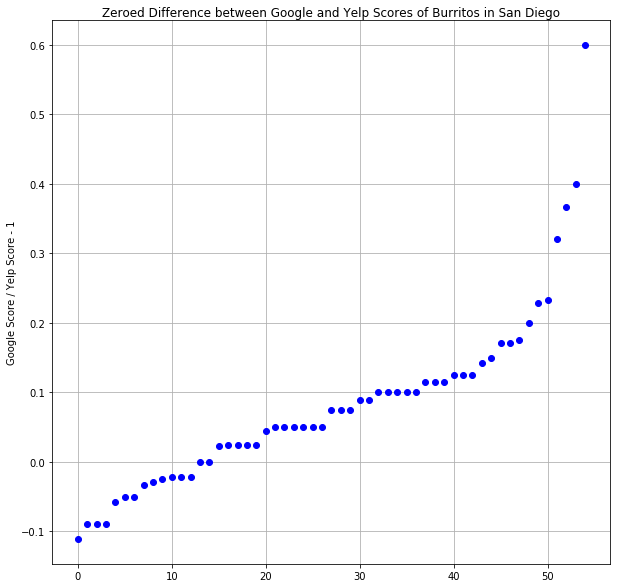
\includegraphics[scale=0.8]{5a}
I have noticed a trend with Google reviews that the mean score of most food places, especially in San Francisco, tend to be around 4. I have also seen the Yelp reviewers are also more parsimonious when reviewing food. Therefore, I was curious about how much of a bonus (if it actually is a bonus) do Google reviews have over Yelp reviews.
\\
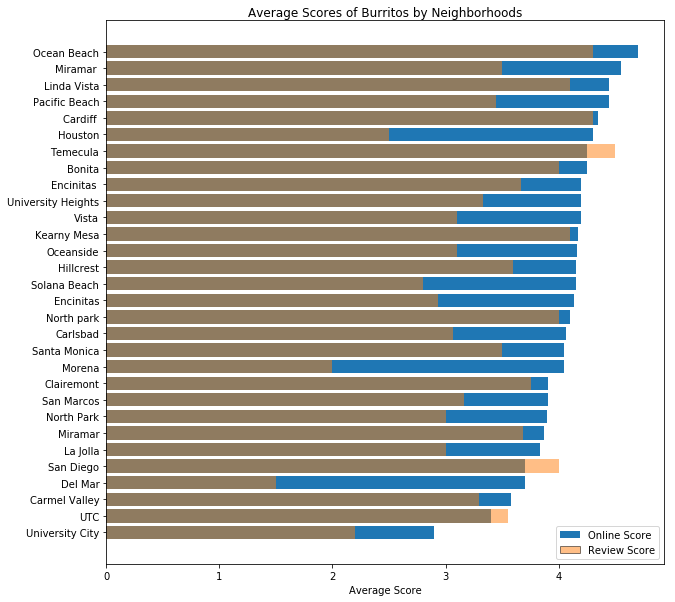
\includegraphics[scale=0.8]{5b}
From the above question, a logical step would be to ask how good are the tastebuds of people who review food on Google and Yelp compared to the people participating in this study. It was interesting to see that there is a large difference between online reviews scores and the scores from this study which could be due to the people participating in study being seasoned burrito eaters who have much higher standards than the general public. 
\\
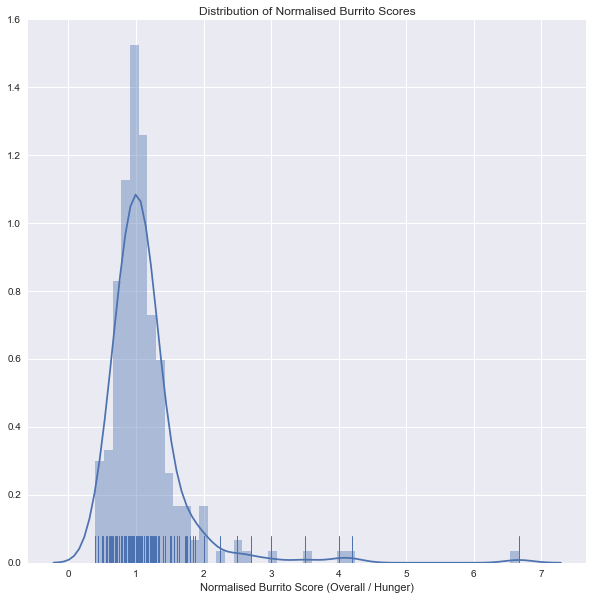
\includegraphics[scale=0.8]{5c}
I feel that I am an impartial judge when it comes to food regardless of my state of hunger as long as I am not too full but I know intuitively that I am likely to be quite subjective. Since the reviewers stated their hunger levels, it would be good to figure how often hunger plays a substantial role in improving the taste of food among the reviewers so I can judge the quality of their recommendations. 
\newline \\
(P.S. Working on this has me extremely hungry $>.<$)

\end{document}